
\documentclass[12pt,a4paper]{article}
\usepackage[left=3.00cm, right=2.00cm, bottom=2.00cm, top=3.00cm]{geometry}
\usepackage{graphics}
\begin{document}
\title{Postman dan Swagger}
\maketitle
\begin{enumerate}
\item Fransiscus Ivan Martongam      1164039 \\
\item Lalita Chandiany Adiputri      1164043\\
\item Eko Cahyono Putro              1164035\\
\item Lidwina Triniska Gulo          1164044\\
\item Sulpadianti Bunyamin           1164096\\
\end{enumerate}

\section{Pengertian Postman}
Postman merupakan sebuah software yang memuat fungsi lengkap pengembangan sistem dalam mengirimkan dan menerima respon server. Software ini mendukung pengembangan sistem REST API dengan mengklasifikasi request berdasarkan request method, URL dan parameter-parameter request. Postman juga adalah sebuah aplikasi (berupa plugin) untuk browser chrome, fungsinya adalah sebagai REST Client atau istilahnya adalah aplikasi yang digunakan untuk melakukan uji coba REST API yang telah kita buat.

\section{Fungsi dari postman}
Menurut Arianto M A, DKK(2016), Sebuah aplikasi yang digunakan untuk melakukan uji coba REST API yang telah kita buat. Fungsi Postman adalah untuk pengecekan web service. Postman dapat menampilkan hasil dari HTTP request yang kompleks sekalipun dengan cepat. Postman muncul sebagai add-on dari chrome namun sekarang sudah menjadi aplikasi native. Postman memudahkan untuk menguji, mengembangkan dan API (Application Programmin Interface) dokumen dengan memungkinkan pengguna untuk dengan cepat mengumpulkan baik permintaan HTTP sederhana dan kompleks

\section{cara instal postman}
Postman for Chrome (aplikasi Postman sebelumnya merupakan ekstensi Chrome App atau aplikasi yang menginduk pada Chrome).
Cara menginstal Postman untuk menginstal Postman versi native pada sistem operasi Ubuntu/Debian yaitu 
Buka terminal lalu unduh atau donwload paket instalasi Postman dengan mengunakan perintah wge,
kemudia Ekstrak file instalasi Postman tersebut ke direktori /optsudo tar -xzf postman.tar.gz -C /opt.
setelah itu dapat menghapus file instalasinya (opsional)dengan cara rm postman.tar.gz


\section{membuat shortcut Postman}
Berikut tata cara untuk membuat shortcut pada start menu postman.  Ketik perintah - perintah berikut dibawah ini:
cat > ~/.local/share/applications/postman.desktop <<EOL
[Desktop Entry]
Encoding=UTF-8
Name=Postman
Exec=postman
Icon=/opt/Postman/resources/app/assets/icon.png
Terminal=false
Type=Application
Categories=Development;
EOL

Sekarang untuk membuka aplikasi yang ada pada Postman , cukup hanya dengan melakukan klik pada shortcut pada start - menu. 

\section{Cara Penggunaan Postman}
Berikut cara penggunaan Postman : Buat sebuah file baru pada direktori root webserver dengan nama: contoh-api-sederhana.php .Kemudian ketikan kode PHP berikut ke dalam file contoh-api-sederhana.php. Berikut kode untuk membuat file:

\begin{figure}[ht]
\centerline{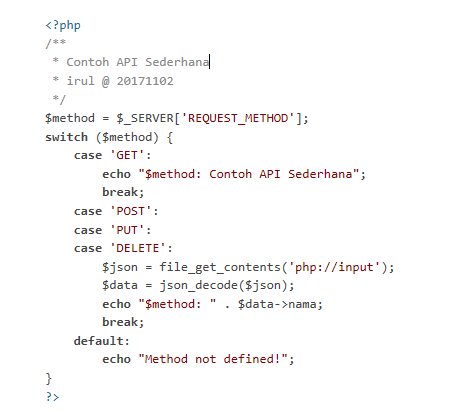
\includegraphics[width=1\textwidth]{figures/3contohapi.PNG}}

\caption{Contoh Api Sederhana} 
\label{api}
\end{figure}

pada gambar \ref{api} menjelaskan tentang contoh api.

Pada file contoh-api-sederhana.php, dapat didefinisikan satu buah API dengan empat Http Request Method yang berbeda. Berikut daftar method dan alamat url yang nanti akan kita uji menggunakan Postman:
•	GET => /contoh-api-sederhana.php
•	POST => /contoh-api-sederhana.php
•	PUT => /contoh-api-sederhana.php
•	DELETE => /contoh-api-sederhana.php
Kita dapat menguji salah satu API di atas menggunakan browser, salah satunya, menggunakan method GET, browser akan mengirimkan data ke server menggunakan method GET.

\section{Implementasi Postman}
Implementasi tidak hanya aktivitas, melainkan suatu kegiatan yang terencana untuk mencapai
tujuan kegiatan. Tahap implementasi pada penelitian ini tidak dilakukan hanya dalam satu proses,
Tetapi dilakukan dalam beberapa sub proses yaitu membangun lingkungan pengembangan sistem, 
mendesain struktur table, function dan stored procedure pada database, mengembangkan sistem back-end (coding) 
dan menyesuaikan dengan database, dan mendesain struktur rewrite pada web server. 

\section{Pengujian}
Untuk memastikan bahwa sistem berjalan sesuai dengan rencana pengembangan sistem dan proses bisnis yang difasilitasi, diperlukan sebuah skenario pengujian sistem. Pada penelitian ini, pengujian akan dilakukan dengan menggunakan software Postman dan dibagi menjadi tiga skenario pengujian, yaitu: Pengujian otentikasi token untuk memastikan prinsip REST terpenuhi, pengujian dengan metode equivalent partitioning untuk memastikan nilai-nilai masukan sesuai dengan rencana pengembangan sistem, pengujian fungsional untuk memastikan setiap titik akses API.

\subsection{Pengujian otentikasi token}
Pengujian  otentikasi token dilakukan pada load-balanced server dengan jumlah back-end server sebanyak tiga virtual server yang diklasifikasi berdasarkan port jaringan. Pengujian  metode equivalent partitioning akan mengelompokkan nilai masukan ke dalam kelas- kelas kemudian diuji dalam kasus-kasus tertentu. Pengujian fungsional dilakukan secara langsung setiap titik akses sistem API yang telah dibuat. 

\subsection {Pengujian dengan metode equivalent partitioning}
Pengujian dengan menggunakan metode equivalent partitioning ini untuk memastikan nilai-nilai masukan sesuai dengan rencana pengembangan sistem. Pengujian ini akan mengelompokkan nilai masukan ke dalam kelaskelas batasan nilai untuk kemudian diuji dalam kasus-kasus tertentu. Rencana pengujian metode ini meliputi validasi path, validasi request method, validasi token, kesesuaian tipe data dan validasi nilai.


\end{document}
